% 相反数的定义及函数图象
\begin{frame}{1.3 相反数}
\begin{definition}
\textbf{\textcolor{orange}{只有正负号不同的两个数称互为相反数(opposite number)。\\
我们规定: 0 的相反数是0 .}}
\end{definition}
\begin{columns}
\column{0.5\textwidth}
\begin{itemize}
    \item \textbf{数学表达式}:  $a + b = 0$
    \item \textbf{函数定义}:  $f(x) = -x$
    \item \textbf{定义域}: $x \in \mathbb{R}$
    \item \textbf{值域}: $y \in \mathbb{R}$
    \item \textbf{对称性}: 关于原点中心对称
\end{itemize}

\column{0.5\textwidth}
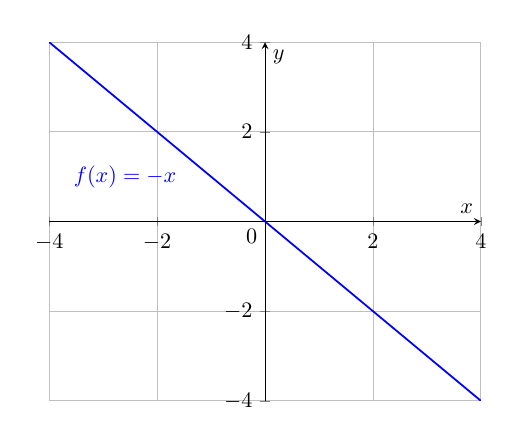
\begin{tikzpicture}[scale=0.8]
\begin{axis}[
    axis lines=middle,
    xlabel=$x$, ylabel=$y$,
    xmin=-4, xmax=4, ymin=-4, ymax=4,
    samples=500,
    grid=both,
    restrict y to domain=-10:10,
]
\addplot[blue, thick] {-x};
\node[black] at (0,0) [below left] {0};
\node[blue] at (-1.5,1) [left] {$f(x)=-x$};
\end{axis}
\end{tikzpicture}
\end{columns}
\end{frame}

% 倒数的定义及函数图象
\begin{frame}{倒数的定义及函数图象}
\begin{definition}
\textbf{\textcolor{orange}{乘积为1的两个数互为倒数。\\
注意:0没有倒数。}}
\end{definition}
\begin{columns}
\column{0.5\textwidth}
\begin{itemize}
    \item \textbf{数学表达式}:  $a \cdot b = 1$
    \item \textbf{函数定义}:  $f(x) = \dfrac{1}{x}$
    \item \textbf{定义域}: $x \in \mathbb{R}, x \neq 0$
    \item \textbf{值域}: $y \in \mathbb{R}, y \neq 0$
    \item \textbf{对称性}: 关于原点中心对称
\end{itemize}

\column{0.5\textwidth}
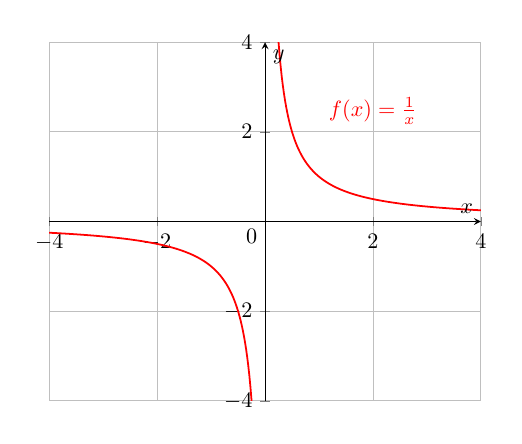
\begin{tikzpicture}[scale=0.8]
\begin{axis}[
    axis lines=middle,
    xlabel=$x$, ylabel=$y$,
    xmin=-4, xmax=4, ymin=-4, ymax=4,
    samples=500,
    grid=both,
    restrict y to domain=-10:10,
]
\addplot[red, thick] {1/x};
\node[black] at (0,0) [below left] {0};
\node[red] at (2,2) [above] {$f(x)=\frac{1}{x}$};
\end{axis}
\end{tikzpicture}
\end{columns}
\end{frame}

% 相反数与倒数的比较
\begin{frame}{相反数与倒数的比较}
\begin{columns}
\column{0.5\textwidth}
\begin{itemize}
    \item \textbf{相反数的表达式}:  $a + b = 0$
    \item \textbf{倒数的表达式}:  $a \cdot b = 1$
    \item \textbf{对称性}: 相反数与倒数均关于原点中心对称
\end{itemize}

\column{0.5\textwidth}
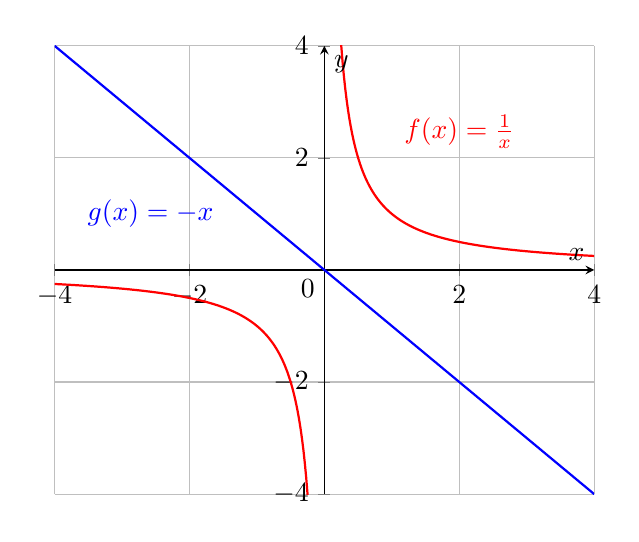
\begin{tikzpicture}[scale=1]
\begin{axis}[
    axis lines=middle,
    xlabel=$x$, ylabel=$y$,
    xmin=-4, xmax=4, ymin=-4, ymax=4,
    samples=500,
    grid=both,
    restrict y to domain=-10:10,
]
\addplot[red, thick] {1/x};
\addplot[blue, thick] {-x};
\node[black] at (0,0) [below left] {0};
\node[red] at (2,2) [above] {$f(x)=\frac{1}{x}$};
\node[blue] at (-1.5,1) [left] {$g(x)=-x$};
\end{axis}
\end{tikzpicture}
\end{columns}
\end{frame}